\documentclass{article}
\usepackage[usenames,dvipsnames]{color} % Required for custom colors
\usepackage{graphicx} % Required to insert images
\usepackage{listings} % Required for insertion of code
\usepackage{amsmath} % Required for some math formulas
\usepackage{enumitem} % Required for customed enum
\usepackage{url} % Auto line break in URL
\usepackage{tabularx} % Auto line break in tabular


\def\UrlBreaks{\do\[\do\\\do\]\do\^\do\_\do\`\do\.\do\@\do\\\do\/\do\!\do\_\do\|\do\;\do\>\do\]\do\)\do\,\do\?\do\'\do+\do\=\do\#}

\usepackage{hyperref} % add clickable link to contents
\hypersetup {
    colorlinks = false, % links colored or not
    hidelinks = true, % border
    linkcolor = blue, % color TOC links in blue
    urlcolor = red, % color URLs in red
    linktoc = all % 'all' will create links for everything in the TOC
}

% Uncomment the lines below if you wish to use Chinese characters
\usepackage{fontspec}  % Chinese characters support
\usepackage{indentfirst} % Add indent at the first paragraph
\XeTeXlinebreaklocale "zh" % Automatic line break
\XeTeXlinebreakskip = 0pt plus 1pt % Automatic line break
% \setmainfont{STSong} % Use a Chinese font
% \setmainfont[Path = ./]{AdobeSongStd-Light.otf} % use font in ./
\setmainfont[Path = ./]{AdobeFangsongStd-Regular.otf}

% Use Chinese for figure name
\renewcommand\figurename{图}

% Use Chinese for contents name
\renewcommand\contentsname{目录}

% Use Chinese for table name
\renewcommand\tablename{表}

% contents depth
\setcounter{tocdepth}{4}

% numbered paragraph
\setcounter{secnumdepth}{4}

%----------------------------------------------------------------------------------------
%	TITLE SECTION
%----------------------------------------------------------------------------------------

\newcommand{\horrule}[1]{\rule{\linewidth}{#1}} % Create horizontal rule command with 1 argument of height

\title{	
\normalfont \normalsize 
% \textsc{university, school or department name} \\ [25pt] % Your university, school and/or department name(s)
\horrule{0.5pt} \\[0.4cm] % Thin top horizontal rule
\huge 32位MIPS处理器实验需求文档 \\ % The assignment title
\horrule{2pt} \\[0.5cm] % Thick bottom horizontal rule
}

\author{Cache小组} % Your name

\date{\normalsize\the\year 年\the\month 月\the\day 日} % Today's date or a custom date




% document begin
\begin{document}
\maketitle % Print the title

\tableofcontents % Print the contents

\newpage % blank after contents

\section{引言}
    \subsection{编写的目}
        计原32位MIPS实验是在计原16位大实验的基础上的扩展。
        在实验原理方面与多门课程相结合,涉及到操作系统、软件工程、编译原理等等多个方面,
        实验初期学习曲线较陡,在原理方面比较难以掌控。
        在编程实现方面涉及到大规模VHDL代码的书写,需要对数字逻辑设计有比较清晰的思路,工作量非常大。

        因此,为控制整个开发过程,明确项目需求与目标,编写此需求文档。 

        文档预期读者为任务提出者:刘卫东老师、白晓颖老师。
    \subsection{背景}
        系统名称:32位MIPS处理器

        任务提出者:
        $
        \begin{minipage}[t]{0.9\linewidth}
        计原课:刘卫东老师

        软工课:白晓颖老师
        \end{minipage}
        $

        开发者:
        $
        \begin{minipage}[t]{0.9\linewidth}
        计23 李天润

        计23 胡津铭

        计23 孙皓
        \end{minipage}
        $

    \subsection{定义}
        以下是此次32位MIPS实验中需要用到的专业名词定义
        \begin{longtable}{|p{0.3\linewidth}|p{0.5\linewidth}|}
        \caption{定义列表}
        \hline
        名词 & 描述 \\
        \hline
        MIPS & 无内部互锁流水级的微处理器 \\
        \hline
        CPU &  中央处理器\\
        \hline
        CP0 & 协处理器0 \\
        \hline
        MMU & 内存管理单元 \\
        \hline
        TLB & 页表后备缓冲 \\
        \hline
        ALU & 算术逻辑单元 \\
        \hline
        RAM & 存储程序的硬件,断电不保存信息 \\
        \hline
        ROM & 存储程序的硬件,断电可保存信息 \\
        \hline
        Flash & 存储程序的硬件,断电可保存信息,实验中用作硬盘 \\
        \hline
        Flash & 主板上的启动程序,负责初始化硬件引导操作系统 \\
        \hline
        Flash & 一段特殊程序,将操作系统从Flash中加载到内存中,并且开始执行 \\
        \hline
        \end{longtable}

    \subsection{参考资料}
        实验指导文档

        OsLab实验参考文档

        贾开Report

        《计算机组成和设计硬件/软件接口》

        《See MIPS Run》



\section{功能需求}
    \subsection{CPU}
        CPU整体工作流程图
        \begin{figure}[!hbp]
            \centering
            \caption{CPU各阶段转换图}
            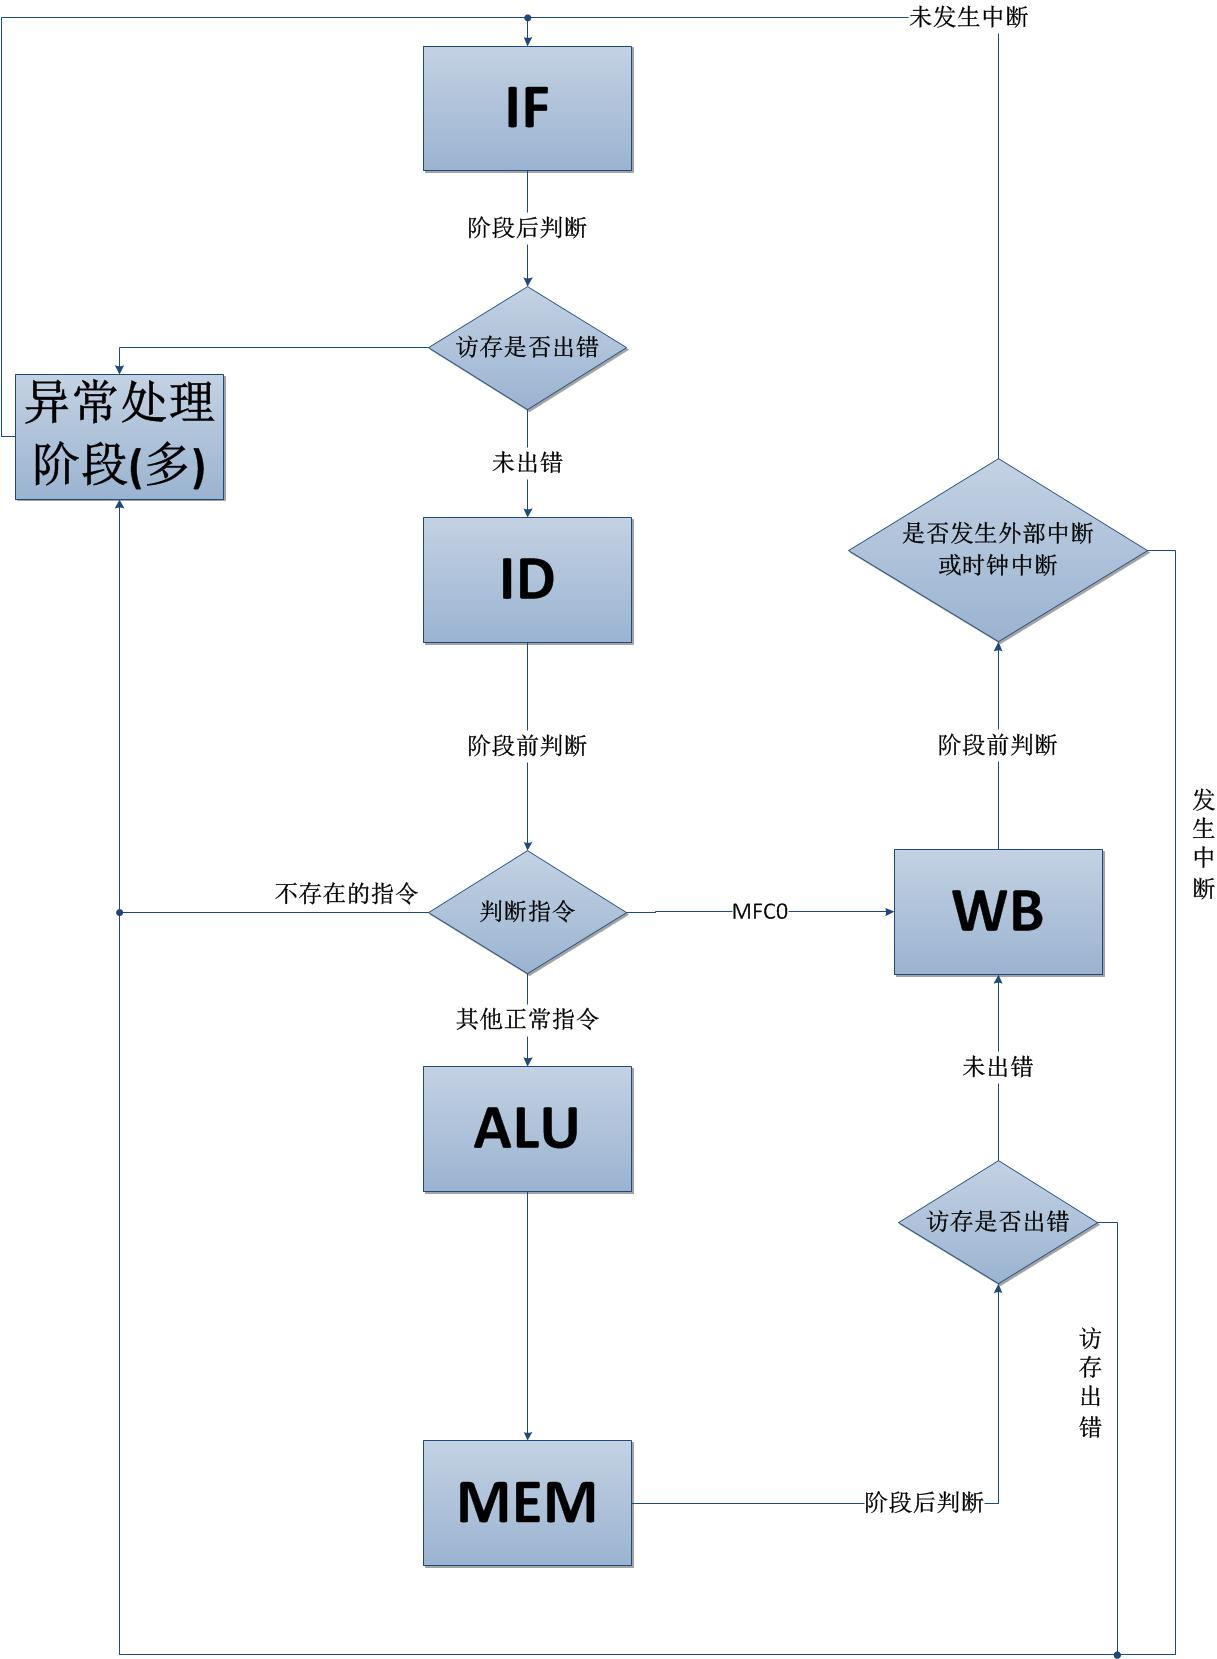
\includegraphics[width=0.75\textwidth]{chart/Stages.jpg}
        \end{figure}
                
        \subsubsection{ALU}
            功能需求:
            \begin{enumerate}
            \item
            完成数据和地址的算术、逻辑和移位运算,%
            输入两个数据根据ALUOp得出输出结果。
            \item
            根据指令系统的需求,完成指令系统中乘法之外的算术指令。
            \end{enumerate}

            实现方式:
            \begin{enumerate}
            \item
            ALU两个输入数据,ALUOp目前整理出9种运算。
            \item
            输出最终运算结果,三个标志位。
            \end{enumerate}

        \subsubsection{乘法器}
            功能需求:
            \begin{enumerate}
            \item
            完成乘法功能,结果保存在LO和HI寄存器中,可以通过MT和MF类指令访问和修改计算结果。
            \end{enumerate}

            实现方式:
            \begin{enumerate}
            \item
            使用IPCore实现。
            \item
            直接与主ALU相结合,在ALUOp中加入乘法的操作码,实现乘法的计算。
            \item
            乘法指令需要的计算时间较长,无法在一个时钟上升沿中完成计算。但是由于是多周期CPU,
            指令执行的控制过程比较灵活,可以在乘法指令时增加多个时钟上升沿,
            当乘法完成后在继续执行下一条指令
            \item
            MFLO,MFHI,MTLO,MTHI,MULT指令查看与修改。
            在ALUOp中也加入支持MTHI、MTLO的操作码,实现对LO和HI的修改。
            同时LO和HI始终处于可读的状态,连接至写回阶段,MFLO与MFHI通过对写回阶段RegValue的控制来实现。
            \end{enumerate}

        \subsubsection{CP0}
            功能需求:

            辅助操作系统对硬件进行管理。
            \begin{enumerate}
            \item
                内存管理:辅助操作系统,完成虚拟地址和物理地址的转换、不同进程之间的内存切换、用户态与内核态内存的分离
            \item
                异常处理:检测指令执行过程中可能出现的异常、对异常进行分类、记录异常出现的指令地址或错误的内存地址
            \item
                外部中断:负责检测外部中断,辅助实现CPU与外设之间的交互

            \end{enumerate}

            实现方式:
            \begin{enumerate}
                \item
                    CP0记录CPU当前状态,通过MFC0、MTC0指令等进行读写操作,与通用寄存器建立联系
                \item
                    在异常状态发生时保存异常的返回地址,异常类型等信息
                \item
                    在内存映射中对TLB表项进行支持,为TLB充填等功能提供硬件支持
                \item
                    CP0寄存器的写方式有两种:
                    \begin{enumerate}
                        \item
                            正常执行状态下,通过MTC0指令,将CP0寄存器编号,CP0写入值,
                            CP0控制信号传递给CP0寄存器,进行写入操作。
                        \item
                            异常状态下,通过异常处理模块到CP0的连接,直接将异常原因、异常指令地址、
                            访存错误地址等信息,写入cause、EPC、BadVAddr寄存器中
                    \end{enumerate}
                \item
                    CP0寄存器的读方式有两种:
                    \begin{enumerate}
                        \item
                            正常执行状态下,通过MFC0指令,将CP0寄存器编号传递给CP0寄存器,
                            之后读取的值通过写回阶段写到通用寄存器中
                        \item
                            针对TLBWI等指令对CP0寄存器的读需求(需要同时读取5个CP0寄存器),
                            将CP0寄存器与TLB相关的直接连接到MMU单元,通过TLBWI的使能信号控制写入TLB
                    \end{enumerate}
            \end{enumerate}

            CP0具体实现方式参照下面两个小节。

            此次实验中需要实现的CP0寄存器见表\ref{table_cp0_reg}

            \begin{table}
            \centering
            \caption{需要实现的CP0寄存器}\label{table_cp0_reg}
            \begin{tabularx}{\textwidth}{|l|l|X|}
            \hline
            序号 & 名称 & 功能 \\
            \hline
            0 & Index & 用于TLBWI指令访问TLB入口的索引序号 \\
            \hline
            1 & EntryLo0 & 作为TLBWI及其他TLB指令接口,管理偶数页入口 \\
            \hline
            2 & EntryLo1 & 作为TLBWI及其他TLB指令接口,管理奇数页入口 \\
            \hline
            3 & EntryHi & TLB异常时,系统将虚拟地址部分写入EntryHi寄存器中用于TLB匹配 \\
            \hline
            4 & BadVAddr & 捕捉最近一次地址错误或TLB异常(重填、失效、修改)时的虚拟地址 \\
            \hline
            5 & Count & 每隔一个时钟周期增加1,用作计时器,并可使能控制 \\
            \hline
            6 & Compare & 当Count值与Compare相等时,SI\_TimerInt 引脚是变高电平直到有数值写入Compare,用于定时中断 \\
            \hline
            7 & Status & 表示协理器的操作模式、中断使能及诊断状态 \\
            \hline
            8 & Cause & 记录最近依次异常的原因,控制软件中断请求以及中断协理派分的向量 \\
            \hline
            9 & EPC & 存储异常处理之后程序恢复执行的地址 \\
            \hline
            10 & EBase & 识别多协理器系统中不同的协理器异常向量的基地址 \\
            \hline
            \end{tabularx}
            \end{table}

        \subsubsection{MMU与TLB}
            功能需求:
            \begin{enumerate}
            \item
                实现虚拟地址(线性地址)到物理地址的转换。% 
                只对部分地址% 
                ([0x20000000$\sim$0x80000000]和[0xC0000000$\sim$0xFFFFFFFF])% 
                进行地址映射,其余部分直接映射。
            \item
                实现内核态与用户态内存的区分。
            \item
                实现相对应的异常处理:TLBS、TLBL、TLB Modified。
            \end{enumerate}

            实现方式:
            \begin{enumerate}
            \item
                \begin{figure}[!hbp]
                    \centering
                    \caption{TLB电路结构}
                    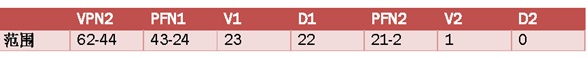
\includegraphics[width=0.9\textwidth]{chart/TLB.jpg}
                \end{figure}

                \begin{figure}[!hbp]
                    \centering
                    \caption{内存访问流程图}
                    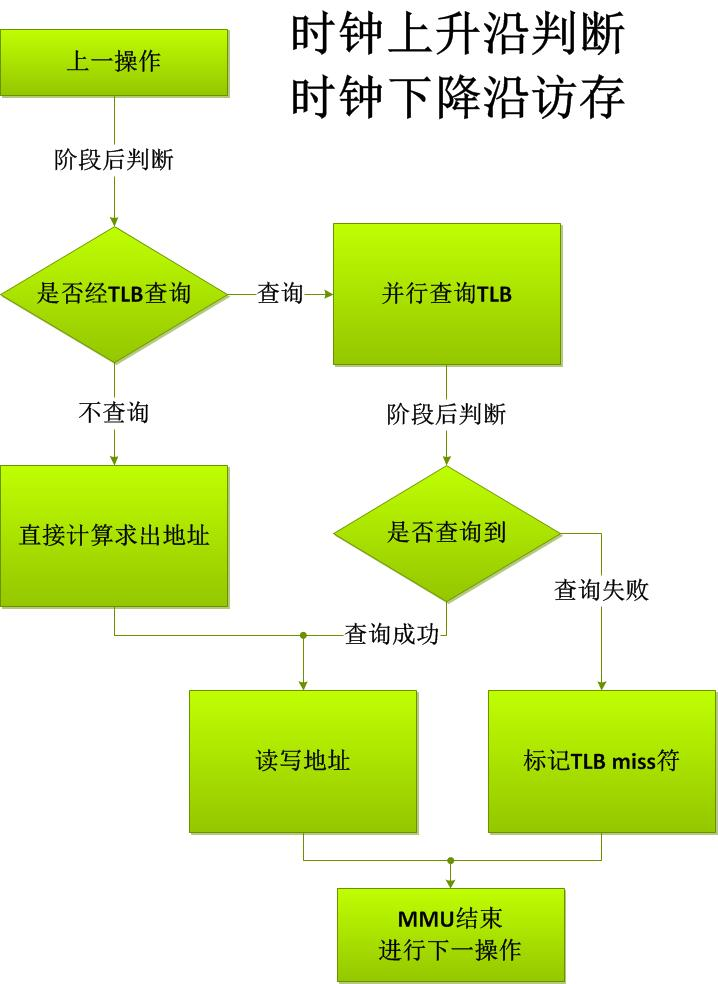
\includegraphics[width=0.4\textwidth]{chart/Memory.jpg}
                \end{figure}
                
                \begin{enumerate}
                \item
                    TLB共16项,每项可以将连续两个虚页映射到两个不同的物理页,相当于可以处理32个页
                \item
                    虚拟地址高19位作为虚页号VPN进行选择TLB表项,第20位通过奇偶判断,选择两个物理页之一
                \item
                    出于简化的考虑,不维护进程号ASID、全局标记G,默认所有G均为1,只维护每个物理地址的D标记
                \end{enumerate}

            \item
                硬件支持:
                \begin{enumerate}
                \item
                    虚拟地址高19位在TLB表项中并行查询EntryHi部分。
                \item
                    如果查找到,根据第20位选择EntryLo,直接与低12位结合得到真实的物理地址。
                \item
                    如果未查找到,触发TLBMiss异常:%
                    设置Cause寄存器中的ExcCode为TLB异常,%
                    EPC寄存器为当前指令的地址,%
                    BadvAddr寄存器为错误的地址,%
                    之后触发一个异常,PC跳转到EBase的异常处理基地址,%
                    之后由操作系统接管。
                \item
                    对于地址不对齐异常,在内存映射阶段对虚拟地址offset部分最低两位进行检测%
                    如果不为00,则触发地址不对齐异常,交由操作系统处理
                \end{enumerate}
            \item
                操作系统:
                \begin{enumerate}
                \item
                    进入异常处理向量(trap/vector.S)。
                \item
                    跳转到处理函数部分(trap/exception.S)。
                \item
                    先保存异常现场,之后进入mips\_trap函数(trap/trap.c)。
                \item
                    根据cause寄存器的值进行分类,调用handle\_tlbmiss函数。
                \item
                    得到异常地址对应的物理页号,%
                    之后进行tlb\_refill(include/thumips\_tlb.h)。
                \item
                    操作系统维护index,%
                    写EntryLo0、EntryLo1、EntryHi、 PageMask、Index五个寄存器,%
                    之后用tlbwi写到TLB的第Index项。%
                    此处需要硬件提供MTC0、MFC0、TLBWI指令的支持。
                \item
                    异常返回,重新执行取地址命令。%
                \end{enumerate}
            \end{enumerate}

        \subsubsection{异常中断处理}
            功能需求:
            \begin{enumerate}
            \item
            实现对异常和外部中断的处理。
            \item
            实现的异常有内存访问异常、地址不对齐异常、%
            系统调用、未定义的指令异常、未定义的寄存器异常。
            \item
            外部中断:键盘、通讯端口。
            \end{enumerate}

            实现方式:
            \begin{figure}[!hbp]
                    \centering
                    \caption{异常中断处理流程}
                    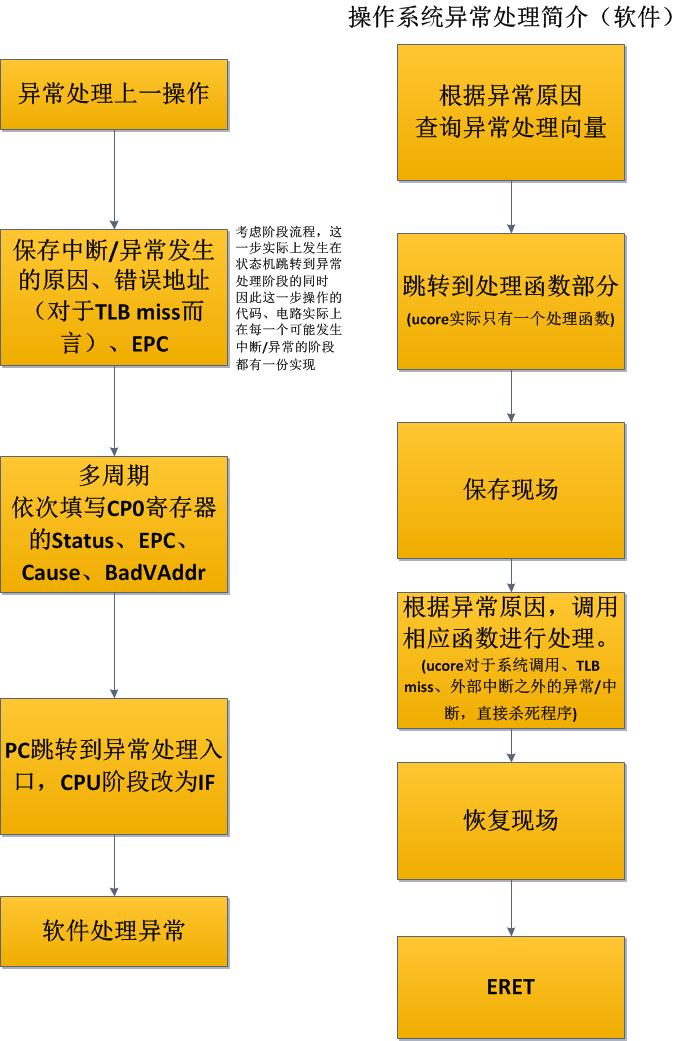
\includegraphics[width=0.5\textwidth]{chart/Exception.jpg}
            \end{figure}
            
            \begin{enumerate}
            \item
            硬件支持
                \begin{enumerate}
                \item
                异常处理,在数据通路上添加异常处理部分,%
                在多周期的任意一个周期检测到异常后,%
                在Cause设置异常代码、
                在EPC寄存器设置异常处理的返回地址,
                将Status寄存器的EXL为设置为1,表示进入内核态处理异常
                之后根据EBase跳转到异常处理向量基地址,%
                之后操作系统接管。
                \item
                外部中断处理,设置外部中断检查信号,外部设备触发时,%
                异步地将检查信号置1;每个指令IF阶段检查该信号,%
                若为1则进入外部中断处理,否则正常执行指令。
                \item
                时钟中断处理。当寄存器Count和Compare寄存器中的数值相等时,%
                触发一个时钟异常,交由操作系统处理。
                \end{enumerate}
            \item
            操作系统
                \begin{enumerate}
                \item
                进入异常处理向量(trap/vector.S)。
                \item
                跳转到处理函数部分(trap/exception.S)。
                \item
                先保存异常现场,之后进入mips\_trap函数(trap/trap.c)。
                \item
                根据cause寄存器的值进行分类,%
                调用interrupt\_handler、syscall等等函数进行处理,%
                如果是地址不对齐异常,未定义的指令或未定义的异常,直接退出。
                \item
                使用ERET指令从异常返回,将EXL位重新设置为0,表示进入用户态
                重新执行取地址命令
                \end{enumerate}
            \end{enumerate}

            \begin{table}
            \centering
            \caption{需要实现的异常}
            \begin{tabular}{|c|c|c|}
            \hline
            异常号 & 异常名 & 描述 \\
            \hline
            0 & Interrupt & 外部中断,异步发生,由硬件引起 \\
            \hline
            1 & TLB Modified & 内存修改异常, 发生在Memory阶段 \\
            \hline
            2 & TLBL & 读未在TLB中映射的内存地址触发的异常 \\
            \hline
            3 & TLBS & 写未在TLB中映射的内存地址触发的异常 \\
            \hline
            4 & ADEL & 读访问一个非对齐地址触发的异常 \\
            \hline
            5 & ADES & 写访问一个非对齐地址触发的异常 \\
            \hline
            8 & SYSCALL & 系统调用 \\
            \hline
            10 & RI & 执行未定义指令异常 \\
            \hline
            11 & Co-Processor Unavailable & 试图访问不存在的协处理器异常 \\
            \hline
            \end{tabular}
            \end{table}

        \subsubsection{其他功能部件}
            \paragraph{PC}
                \mbox{} \\ 

                功能需求:
                \begin{enumerate}
                \item
                实现PC的多种变换方式:正常执行、分支、跳转。
                \item
                实现异常处理时对PC的处理,跳转到异常处理向量部分。
                \end{enumerate}

                实现方式
                \begin{enumerate}
                \item
                通过多路选择器选择ALU的输入数据,与当前PC进行运算%
                实现PC的多种变化方式。
                \item
                针对异常状态、从异常返回两种情况的PC变化,从CP0寄存器中引出EPC与EBase两个地址到PC计算单元。
                通过当前的状态进行判断PC的取值。
                \item
                下一条指令的PC在本条指令的写回阶段得到确定,
                保证在下一条指令的取指令时钟上升沿开始之前,正确送到MMU进行取指令。
                \end{enumerate}

            \paragraph{寄存器堆}
                \mbox{} \\ 

                功能需求:
                \begin{enumerate}
                \item
                实现通用寄存器,以及在数据通路中的读写控制。
                \end{enumerate}

                实现方式
                \begin{enumerate}
                \item
                在CPU中实现寄存器堆并实现读写控制。
                \item
                在解码指令阶段,根据指令的rs、rt、rd位置读取通用寄存器。
                与写回模块相配合,完成寄存器堆的写入
                \end{enumerate}

            \paragraph{串口}
                \mbox{} \\

                功能需求:
                \begin{enumerate}
                \item
                实现与PC机通信,通过计算机键盘输入数据,向计算机输出数据。
                \end{enumerate}

                实现方式
                \begin{enumerate}
                \item
                使用开源的%
                \href{http://www.fpga4fun.com/SerialInterface.html}{ASync transmitter and receiver},%
                通过在每个信号周期内多次采样,并滤波得到稳定的信号。%
                CPLD仅负责TX/RX端口数据的转发,%
                对数据的编码与解码在FPGA中进行。%
                这样设计提高了数据传送的准确率,%
                并且串口数据不需要占用内存数据线,%
                无需处理冲突,简化了设计。%
                数据通信协议在开发过程中设计,有待进一步说明。

                \end{enumerate}
        \subsubsection{扩展部分}
            在开发过程中需要分模块进行测试,因此在开发阶段计划实现一个分模块的测试工具。

            \begin{enumerate}
            \item
            使用仿真工具ModelSim或者Xilinx自带的ISim进行仿真,
            在给定的输入波形下产生对应的输出波形,将输入与输出波形都输出到文件中。
            之后再使用该测试工具(用python或者c++等高级语言实现),对输出与标准输出进行比较,判断该模块是否正常工作。

            \item
            在模块测试阶段,使用Xilinx提供的ipcore生成一块片内RAM,作为临时的存储区域。
            能够做到在一个时钟上升沿内进行读写操作,操作比一般RAM简便。
            由此在MMU和MEM部分未完成的情况下,可以对其他模块进行独立的测试,而且可以进行内存的访问。

            \item
            每个模块正常工作之后,将各个模块进行组合,形成整体的CPU设计,再进行后续调试工作。

            \end{enumerate}
            对于测试工具部分会实时与老师进行沟通,明确老师对于测试工具的要求。

            如果操作系统已经能够在CPU上正常运行,而且距离项目结束还有比较长的时间,则可以考虑对网口进行扩展。


        \subsubsection{指令集与数据通路}
            指令集为标准MIPS系统子集

            实现多周期CPU,针对指令集设计数据通路。
            仿照《软件硬件接口》书中的多周期CPU进行设计,
            在书中7条指令的原型上进行扩展,以支持标准MIPS系统的子集。
            
            指令执行过程主要分为取指、解码、执行、访存、写回五个周期,
            某些指令可能需要其他特殊的周期支持,采用多周期实现比较灵活。

            数据通路包括状态机与控制线设计,每条指令有不同的状态机变化,
            而且对指令进行解码,能够得到相应的控制线。%
            在多周期的不同周期利用控制线对数据通路进行控制,使指令正常执行。
            
            数据通路图比较大,因此不显示在需求文档中。另附图片文件显示。

            
    \subsection{BIOS}
        准备阶段:
        \begin{enumerate}
            \item
                操作系统和其他程序烧写到Flash中%
            \item
                bootasm.S编译出的二进制文件写到ROM中
            \item
                CPU代码烧写到FPGA中。
        \end{enumerate}

        启动阶段:
        \begin{enumerate}
            \item
                从ROM中的bootasm.S启动
            \item
                将Flash中的全部操作系统拷贝到RAM中,然后控制权交给操作系统。
        \end{enumerate}

        操作系统启动阶段:
        \begin{enumerate}
            \item
                bootasm.S工作结束后,进入操作系统entry.S文件中进行寄存器初始化。
            \item
                entry.S:通用寄存器清零,CP0寄存器设置为默认值,异常处理基地址进行初始化,之后跳转到init.c中的kern\_init。
            \item
                kern\_init:完成TLB初始化(全部TLB表项清零),物理内存与虚拟内存的转换页表的初始化(创建初始页表)
            \item
                最后完成操作系统的进程和文件管理系统,至此ucore系统开始正常工作,
        \end{enumerate}
        


\section{性能需求}
    实现多周期CPU,性能上可能与流水线存在一定差距,
    尽量通过良好的内部设计弥补,减小各个模块之间的延时。

    主频目标暂定为$6.25MHz$。

\section{运行环境需求}
    \subsection{设备}

        \begin{table}[!hbp]
        \centering
        \caption{设备与外部接口}
        \begin{tabular}{|l|l|}
        \hline
        环境 & 描述 \\
        \hline
        FPGA & Xilinx Spartan6 xc6slx100 \\
        \hline
        RAM & 32-bit字长, 4块, 共8MB \\
        \hline
        Flash & 16-bit 字长, 共8MB \\
        \hline
        CPLD & 与FPGA相连, 用于I/O \\
        \hline
        串口 & 2个 \\
        \hline
        USB 串口 & 1个 \\
        \hline
        ps/2 接口 & 1个 \\
        \hline
        以太网接口 & 1个 \\
        \hline
        VGA 接口 & 1个 \\
        \hline
        \end{tabular}
        \end{table}

    \subsection{控制}
        控制部分采用串口作为输入设备,%
        如果有需要可以启用实验板上的第二个串口。%


\newpage
\section{附录}
    \subsection{指令系统}

    \begin{table}[!hbp]
    \begin{tabularx}{\textwidth}{|c|X|}
        \hline
        Syntax: & addiu \$d, \$s, \$t \\
        \hline
        Description: & Adds a register and a sign-extended immediate value and stores the result in a register \\
        \hline
        Operation: & \$t=\$s + imm; \\
        \hline
        Encoding: & 0010 00ss ssst tttt iiii iiii iiii iiii \\
        \hline
    \end{tabularx}
    \end{table}

    \begin{table}[!hbp]
    \begin{tabularx}{\textwidth}{|c|X|}
        \hline
        Syntax: & addu \$d, \$s, \$t \\
        \hline
        Description: & Adds two registers and stores the result in a register \\
        \hline
        Operation: & \$d = \$s + \$t; \\
        \hline
        Encoding: & 0000 00ss ssst tttt dddd d000 0010 0001 \\
        \hline
    \end{tabularx}
    \end{table}

    
    \begin{table}[!hbp]
    \begin{tabularx}{\textwidth}{|c|X|}
        \hline
        Syntax: & slt \$d, \$s, \$t \\
        \hline
        Description: & If \$s is less than \$t, \$d is set to one. It gets zero otherwise. \\
        \hline
        Operation: & if \$s < \$t \$d = 1 else \$d = 0; \\
        \hline
        Encoding: & 0000 00ss ssst tttt dddd d000 0010 1010 \\
        \hline
    \end{tabularx}
    \end{table}

    \begin{table}[!hbp]
    \begin{tabularx}{\textwidth}{|c|X|}
        \hline
        Syntax: & slti \$t, \$s, imm \\
        \hline
        Description: & If \$s is less than immediate, \$t is set to one. It gets zero otherwise. \\
        \hline
        Operation: & if \$s < imm \$t = 1 else \$t = 0 \\
        \hline
        Encoding: & 0010 10ss ssst tttt iiii iiii iiii iiii \\
        \hline
    \end{tabularx}
    \end{table}

    \begin{table}[!hbp]
    \begin{tabularx}{\textwidth}{|c|X|}
        \hline
        Syntax: & sltiu \$t, \$s, imm \\
        \hline
        Description: & If \$s is less than the unsigned immediate, \$t is set to one. It gets zero otherwise. \\
        \hline
        Operation: & if \$s < imm \$t = 1 else \$t = 0; \\
        \hline
        Encoding: & 0010 11ss ssst tttt iiii iiii iiii iiii \\
        \hline
    \end{tabularx}
    \end{table}
    
    \begin{table}[!hbp]
    \begin{tabularx}{\textwidth}{|c|X|}
        \hline
        Syntax: & sltu \$d, \$s, \$t \\
        \hline
        Description: & If \$s is less than \$t, \$d is set to one. It gets zero otherwise. \\
        \hline
        Operation: & if \$s < \$t \$d = 1 else \$d = 0; \\
        \hline
        Encoding: & 0000 00ss ssst tttt dddd d000 0010 1011 \\
        \hline
    \end{tabularx}
    \end{table}

    \begin{table}[!hbp]
    \begin{tabularx}{\textwidth}{|c|X|}
        \hline
        Syntax: & subu \$d, \$s, \$t \\
        \hline
        Description: & Subtracts two registers and stores the result in a register \\
        \hline
        Operation: & \$d = \$s - \$t; \\
        \hline
        Encoding: & 0000 00ss ssst tttt dddd d000 0010 0011 \\
        \hline
    \end{tabularx}
    \end{table}

    \begin{table}[!hbp]
    \begin{tabularx}{\textwidth}{|c|X|}
        \hline
        Syntax: & mult \$s, \$t \\
        \hline
        Description: & Multiplies \$s by \$t and stores the result in \$HI|\$LO. \\
        \hline
        Operation: & \$HI|\$LO = \$s * \$t; \\
        \hline
        Encoding: & 0000 00ss ssst tttt 0000 0000 0001 1000 \\
        \hline
    \end{tabularx}
    \end{table}

    \begin{table}[!hbp]
    \begin{tabularx}{\textwidth}{|c|X|}
        \hline
        Syntax: & mflo \$d \\
        \hline
        Description: & The contents of register LO are moved to the specified register. \\
        \hline
        Operation: & \$d = \$LO; \\
        \hline
        Encoding: & 0000 0000 0000 0000 dddd d000 0001 0010 \\
        \hline
    \end{tabularx}
    \end{table}

    \begin{table}[!hbp]
    \begin{tabularx}{\textwidth}{|c|X|}
        \hline
        Syntax: & mfhi \$d \\
        \hline
        Description: & The contents of register HI are moved to the specified register. \\
        \hline
        Operation: & \$d = \$HI; \\
        \hline
        Encoding: & 0000 0000 0000 0000 dddd d000 0001 0000 \\
        \hline
    \end{tabularx}
    \end{table}

    \begin{table}[!hbp]
    \begin{tabularx}{\textwidth}{|c|X|}
        \hline
        Syntax: & mtlo \$s \\
        \hline
        Description: & The contents of register LO are replaced by the specified register. \\
        \hline
        Operation: & \$LO = \$s; \\
        \hline
        Encoding: & 0000 00ss sss0 0000 0000 0000 0001 0011 \\
        \hline
    \end{tabularx}
    \end{table}

    \begin{table}[!hbp]
    \begin{tabularx}{\textwidth}{|c|X|}
        \hline
        Syntax: & mthi \$s \\
        \hline
        Description: & The contents of register HI are replaced by the specified register. \\
        \hline
        Operation: & \$HI = \$s; \\
        \hline
        Encoding: & 0000 00ss sss0 0000 0000 0000 0001 0001 \\
        \hline
    \end{tabularx}
    \end{table}

    \begin{table}[!hbp]
    \begin{tabularx}{\textwidth}{|c|X|}
        \hline
        Syntax: & and \$d, \$s, \$t \\
        \hline
        Description: & Bitwise ands two registers and stores the result in a register. \\
        \hline
        Operation: & \$d = \$s \& \$t; \\
        \hline
        Encoding: & 0000 00ss ssst tttt dddd d000 0010 0100 \\
        \hline
    \end{tabularx}
    \end{table}

    \begin{table}[!hbp]
    \begin{tabularx}{\textwidth}{|c|X|}
        \hline
        Syntax: & andi \$t, \$s, imm \\
        \hline
        Description: & Bitwise ands a register and an immediate value and stores the result in a register. \\
        \hline
        Operation: & \$t = \$s \& imm; \\
        \hline
        Encoding: & 0011 00ss ssst tttt iiii iiii iiii iiii \\
        \hline
    \end{tabularx}
    \end{table}

    \begin{table}[!hbp]
    \begin{tabularx}{\textwidth}{|c|X|}
        \hline
        Syntax: & lui \$t, imm \\
        \hline
        Description: & The immediate value is shifted left 16 bits and stored in the register.
                         The lower 16 bits are zeroes. \\
        \hline
        Operation: & \$t = (imm << 16); \\
        \hline
        Encoding: & 0011 11-- ---t tttt iiii iiii iiii iiii \\
        \hline
    \end{tabularx}
    \end{table}

    \begin{table}[!hbp]
    \begin{tabularx}{\textwidth}{|c|X|}
        \hline
        Syntax: & nor \$d, \$s, \$t \\
        \hline
        Description: & Bitwise logical ors two registers and stores the logical not result in a register. \\
        \hline
        Operation: & \$d = $\sim$ (\$s | \$t); \\
        \hline
        Encoding: & 0000 00ss ssst tttt dddd d000 0010 0111 \\
        \hline
    \end{tabularx}
    \end{table}


    \begin{table}[!hbp]
    \begin{tabularx}{\textwidth}{|c|X|}
        \hline
        Syntax: & or \$d, \$s, \$t \\
        \hline
        Description: & Bitwise logical ors two registers and stores the result in a register. \\
        \hline
        Operation: & \$d = \$s | \$t; \\
        \hline
        Encoding: & 0000 00ss ssst tttt dddd d000 0010 0101 \\
        \hline
    \end{tabularx}
    \end{table}

    \begin{table}[!hbp]
    \begin{tabularx}{\textwidth}{|c|X|}
        \hline
        Syntax: & ori \$t, \$s, imm \\
        \hline
        Description: & Bitwise ors a register and an immediate value and stores the result in a register. \\
        \hline
        Operation: & \$t = \$s | imm; \\
        \hline
        Encoding: & 0011 01ss ssst tttt iiii iiii iiii iiii \\
        \hline
    \end{tabularx}
    \end{table}

    \begin{table}[!hbp]
    \begin{tabularx}{\textwidth}{|c|X|}
        \hline
        Syntax: & ori \$t, \$s, imm \\
        \hline
        Description: & Bitwise ors a register and an immediate value and stores the result in a register. \\
        \hline
        Operation: & \$t = \$s | imm; \\
        \hline
        Encoding: & 0011 01ss ssst tttt iiii iiii iiii iiii \\
        \hline
    \end{tabularx}
    \end{table}

\newpage

\end{document}
